\documentclass[11pt]{article}  % required first line, though can vary;
                               % this says we will use 11-point font,
                               % in the "article" format
\usepackage{mathtools}
\usepackage{listings}
\usepackage{graphicx}
\graphicspath{{image/}}


%\DeclareGraphicsExtensions{.jpg}


% these \setlength etc. lines concern page layout, amount of paragraph
% indentation etc.; beginners should ignore them (but include them)
\setlength{\oddsidemargin}{0.0in}
\setlength{\evensidemargin}{0.0in}
\setlength{\topmargin}{-0.25in}
\setlength{\headheight}{0in}
\setlength{\headsep}{0in}
\setlength{\textwidth}{6.5in}
\setlength{\textheight}{9.25in}
\setlength{\parindent}{0in}
\setlength{\parskip}{2mm}

\begin{document}
\begingroup
    \fontsize{18pt}{25pt}\selectfont

    \begin{center}
    \textbf{Project Forestcover}\\
\begingroup
\fontsize{10pt}{212pt}\selectfont
Team Members
\endgroup
\line(1,0){500}
\end{center}
\endgroup

\section*{Task:}
Predicting forest cover type from cartographic variables. There are 12 features and 7 categories of forest covers. We use randomly picked $75\%$ of the data samples as training data set and the rest $25\%$ for testing. We use three different classification algorithms: aritificial neural networks, ...
\section*{Method 1: ANN}


\subsection*{$\S$ Plain ANN}

\begin{itemize}
\item Structure of the ANN:
We choose to have 3 layers(1 hidden layer), 5 hidden nodes, and 7 output nodes, and use L2 regularization.
\item Choice of the Activation Functions
We use both sigmoid function 

\begin{equation}
S(t) = \frac{1}{1 + e^{-t}}
\end{equation}

and tanh function 
\begin{equation}
T(t) = 1.7159tanh(\frac{2}{3}t)
\end{equation}
as our activation function.
\item Predictiing Results
\begin{itemize}

\item Sigmoid function:

\item Tanh function: 

\end{itemize}

\item An alternative structure: 3 layers(1 hidden layer), 7 hidden nodes, and 7 output nodes, and use L2 regularization. And the predictiing results are the following:
\begin{itemize}

\item Sigmoid function:

\item Tanh function: 
\end{itemize}
\end{itemize}


\subsection*{$\S$ Feature Selected ANN}
Instead of using all 12 features, we decide to use less feature which are relatively independent to each other. We first contructed a feature scatter plot to observe the dependency of features. (we are not sure which one's to delete for now)
%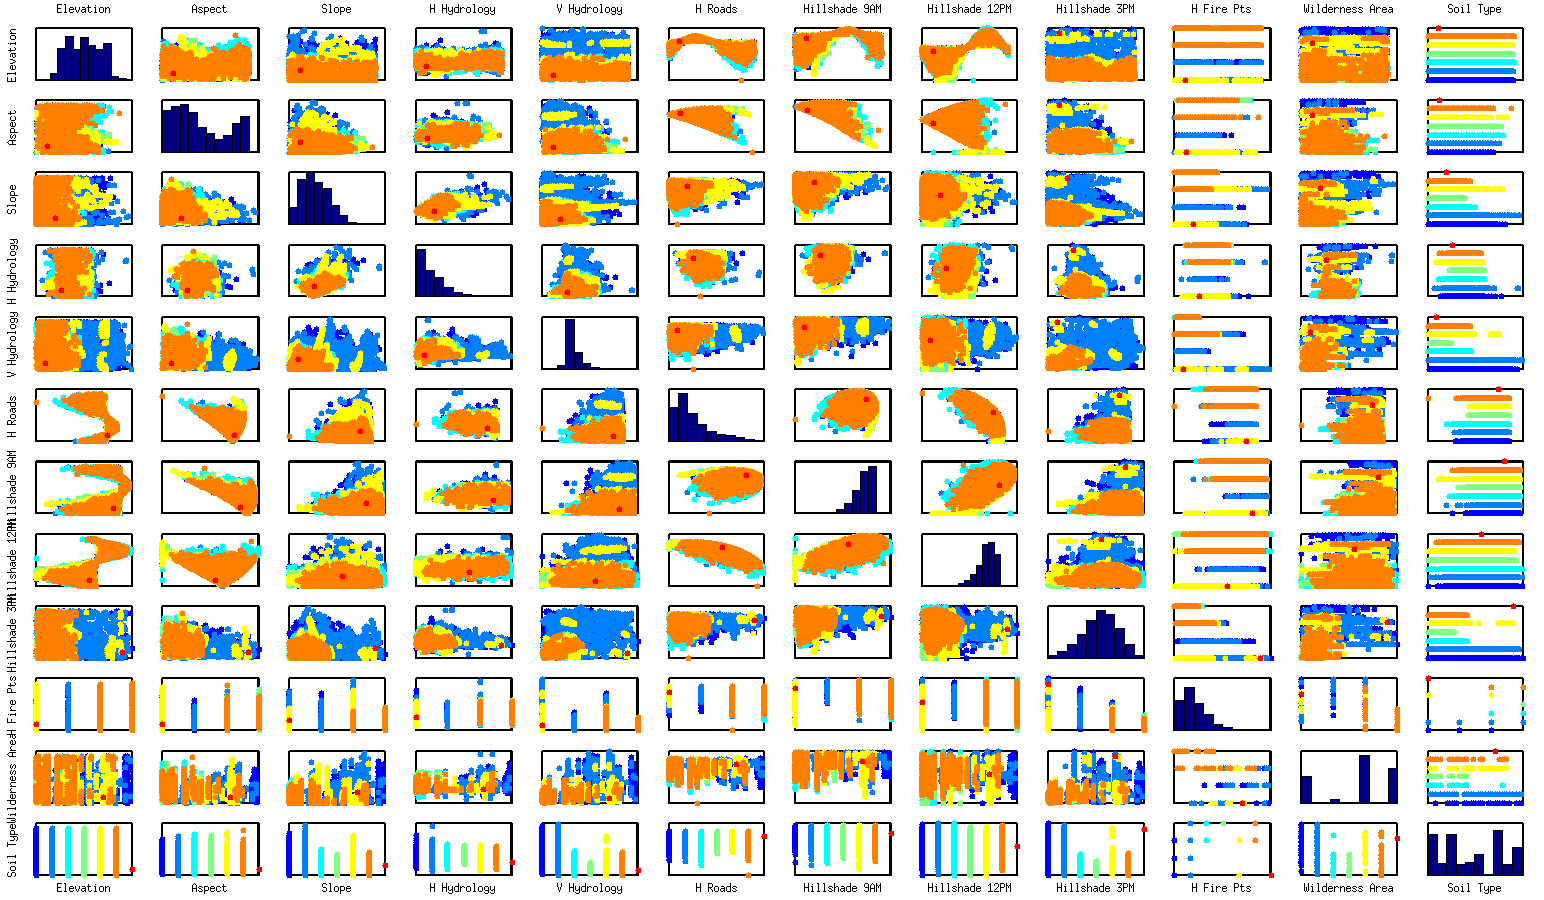
\includegraphics[scale=0.4]{featureScatterPlotMatrixHD}



\begin{itemize}
\item 
\item 
\item 


\end{itemize}





\end{document}
